

\chapter{Authentication}
	
\section{An Attack that doesn’t break Secrecy}
	\begin{center}
		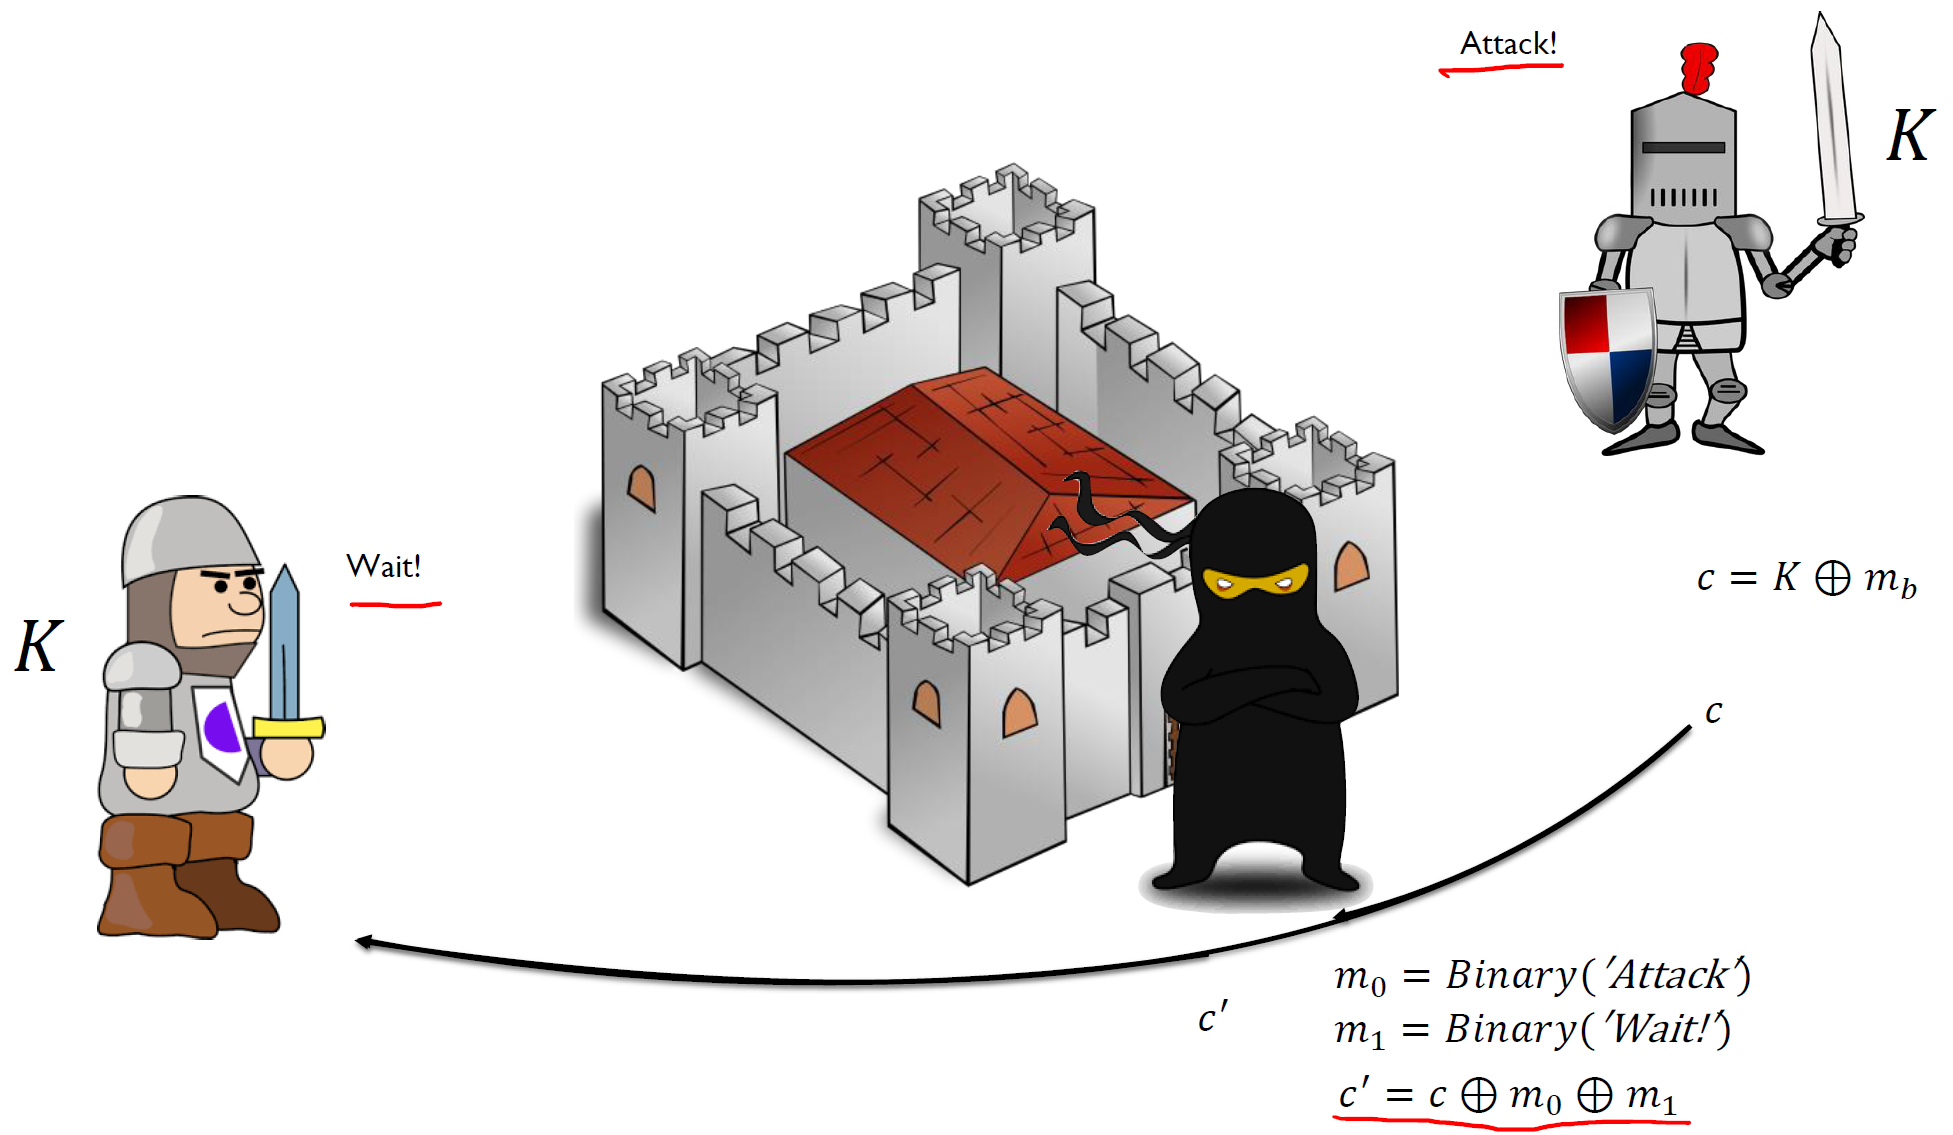
\includegraphics[width=140mm]{Graphics/Authentication/a1.png}
	\end{center}

\section{Message Integrity}
	\begin{itemize}
		\item Need a mechanism to ensure that messages are authentic!
		\item Authentic messages should not be \textit{tamperable}
		\item More examples:
		\begin{itemize}
			\item Bank Transaction
			\item Cookies
		\end{itemize}
		\item Idea: you need to be in possession of a secret to be able to authenticate messages
	\end{itemize}
	\begin{center}
		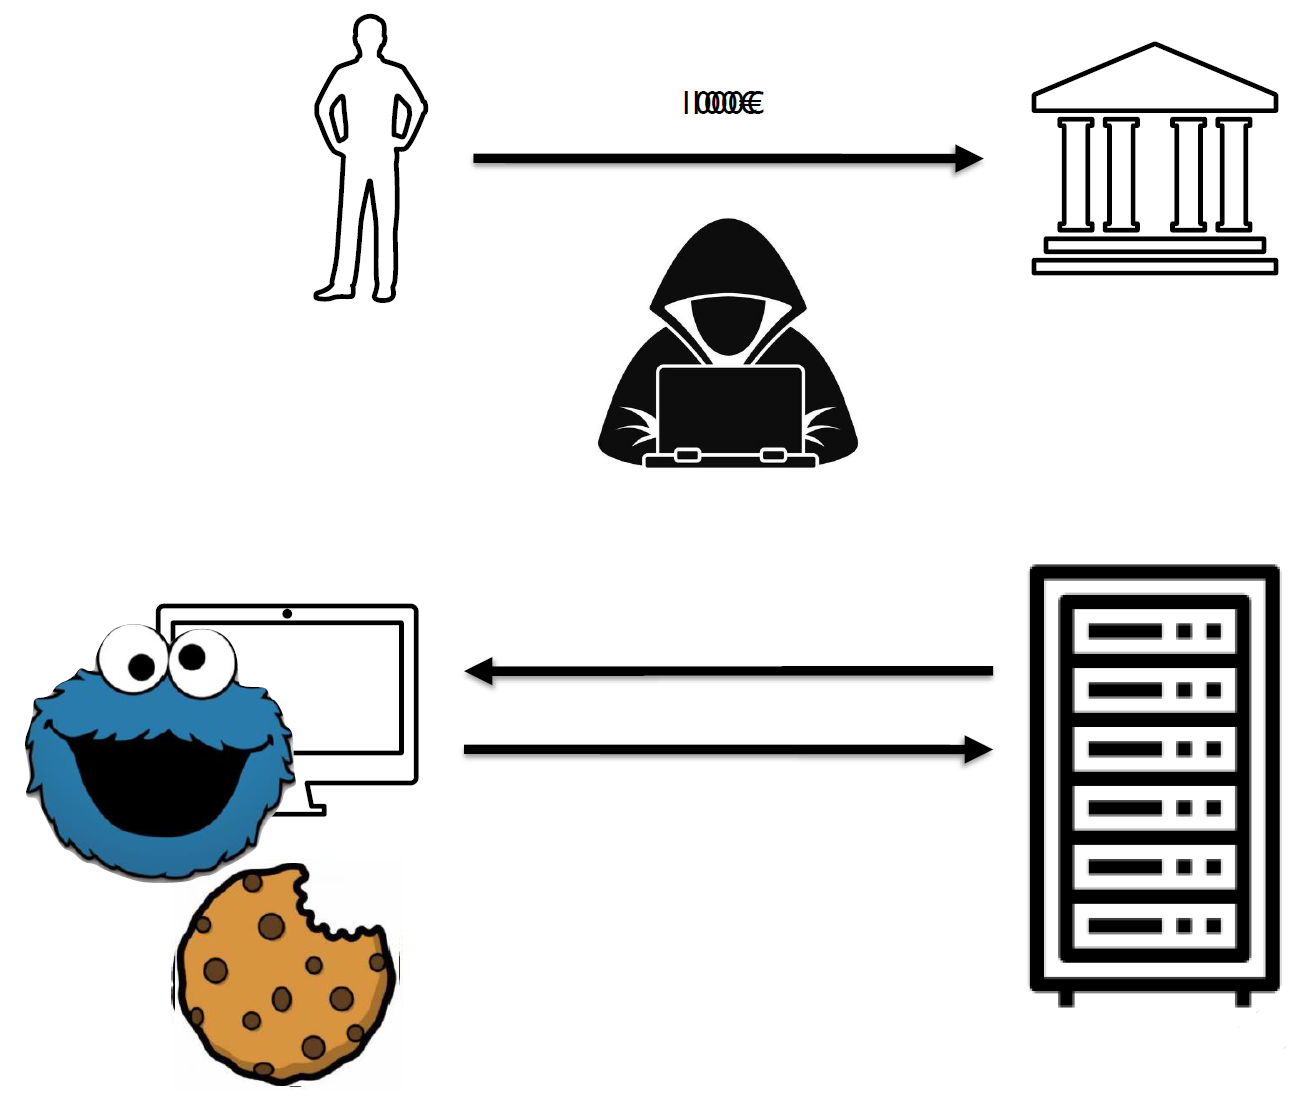
\includegraphics[width=140mm]{Graphics/Authentication/a2.png}
	\end{center}

\section{Message Authentication Codes}
	\textbf{Syntax:} An message authentication code consists of three PPT algorithms: $(Gen,Mac,Verify)$
	\begin{itemize}
		\item $Gen(1^{\lambda})$: A randomized algorithm which takes as input the security parameter $1^{\lambda}$ (encoded in unary) and outputs a key $K$
		\item $Mac(K,m)$: A (possibly randomized) algorithm which takes a key $K$ and message $m$ as input and outputs authentication tag $t$
		\item $Verify(K,m,t)$: A deterministic algorithm which takes as a key $K$, a message $m$ and a tag $t$ as input and outputs a bit $b$
	\end{itemize}
	\textbf{Correctness:} It holds for all $\lambda \in \mathbb{N}$ and all messages $m$ that $Pr[Verify(K,m,Mac(K,m)) = 1] = Pr[Verify(K,m,t) = 1] = 1$, where $K \leftarrow Gen(1^{\lambda})$

\section{Security of Message Authentication Codes}
	\begin{itemize}
		\item How can we formalize security of MACs?
		\item What resources are given to the adversary?
		\begin{itemize}
			\item Real world adversary sees authenticated messages
			\item[$\Rightarrow$] Let adversary choose authenticated messages (as in CPA security)
		\end{itemize}
		\item What is the goal of the adversary?
		\begin{itemize}
			\item Real world: Authenticate a new meaningful message
			\item Better: Authenticate any new message
		\end{itemize}
	\end{itemize}
	
	\begin{definition}[$EUF-CMA$-secure]
		A message authentication code $(Gen,Mac,Verify)$ is existentially unforgeable under adaptive chosen message attacks, or $EUF-CMA$-\textbf{secure}, 
		if it holds for \textbf{every PPT-bounded adversary} $\mathcal{A}$ there exists a negligible function $v$ s.t. for all $\lambda \in \mathcal{N}$
		$$Pr[EUF-CMA_{\mathcal{A}}(\lambda) = 1] < v(\lambda)$$
	\end{definition}
	\begin{center}
		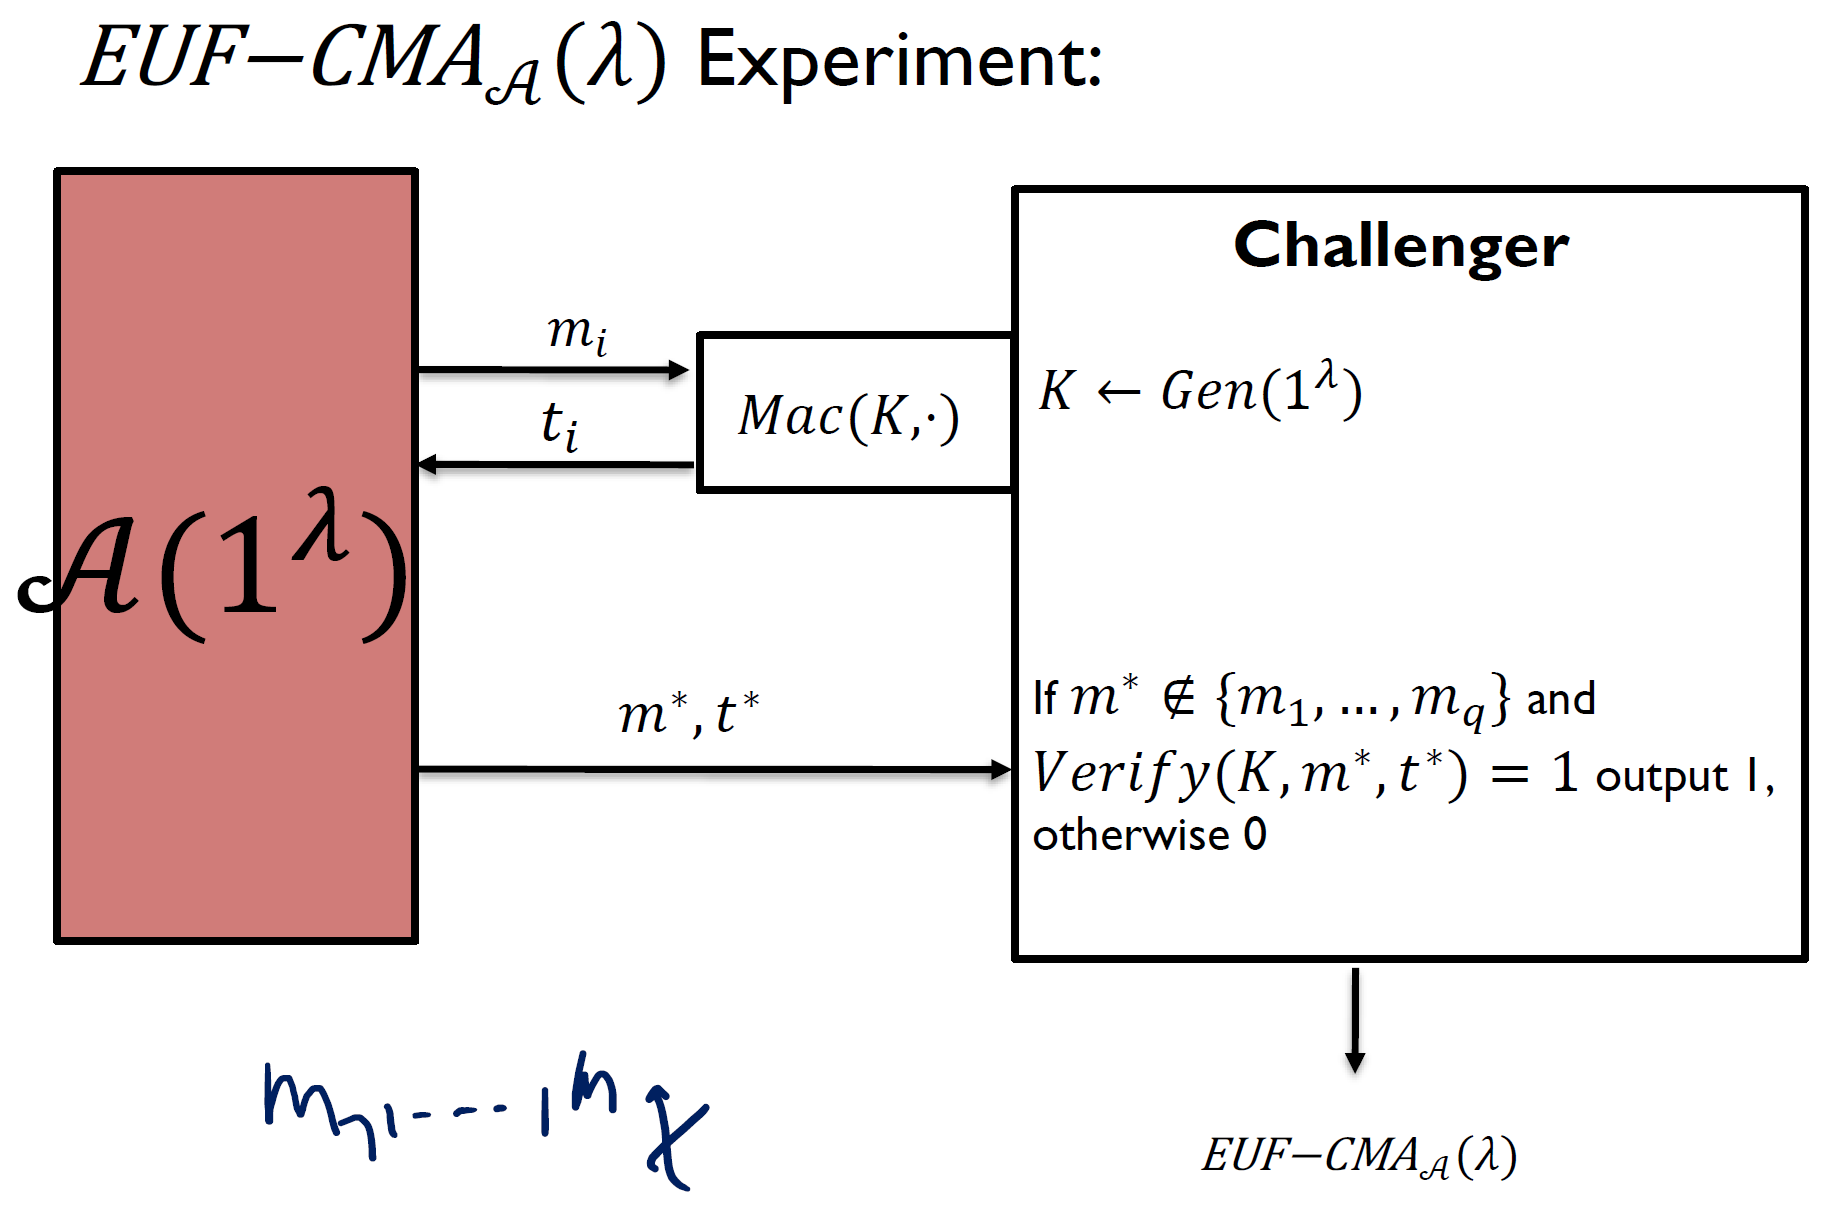
\includegraphics[width=120mm]{Graphics/Authentication/a3.png}\\
	\end{center}

	\begin{definition}[$sEUF-CMA$-secure]
		A message authentication code $(Gen,Mac,Verify)$ is \textbf{strongly} existentially unforgeable under adaptive chosen message attacks, or \textbf{strongly} $EUF-CMA$-\textbf{secure}, 
		if it holds for \textbf{every PPT-bounded adversary} $\mathcal{A}$ there exists a negligible function $v$ s.t. for all $\lambda \in \mathcal{N}$
		$$Pr[sEUF-CMA_{\mathcal{A}}(\lambda) = 1] < v(\lambda)$$
	\end{definition}
	\begin{center}
		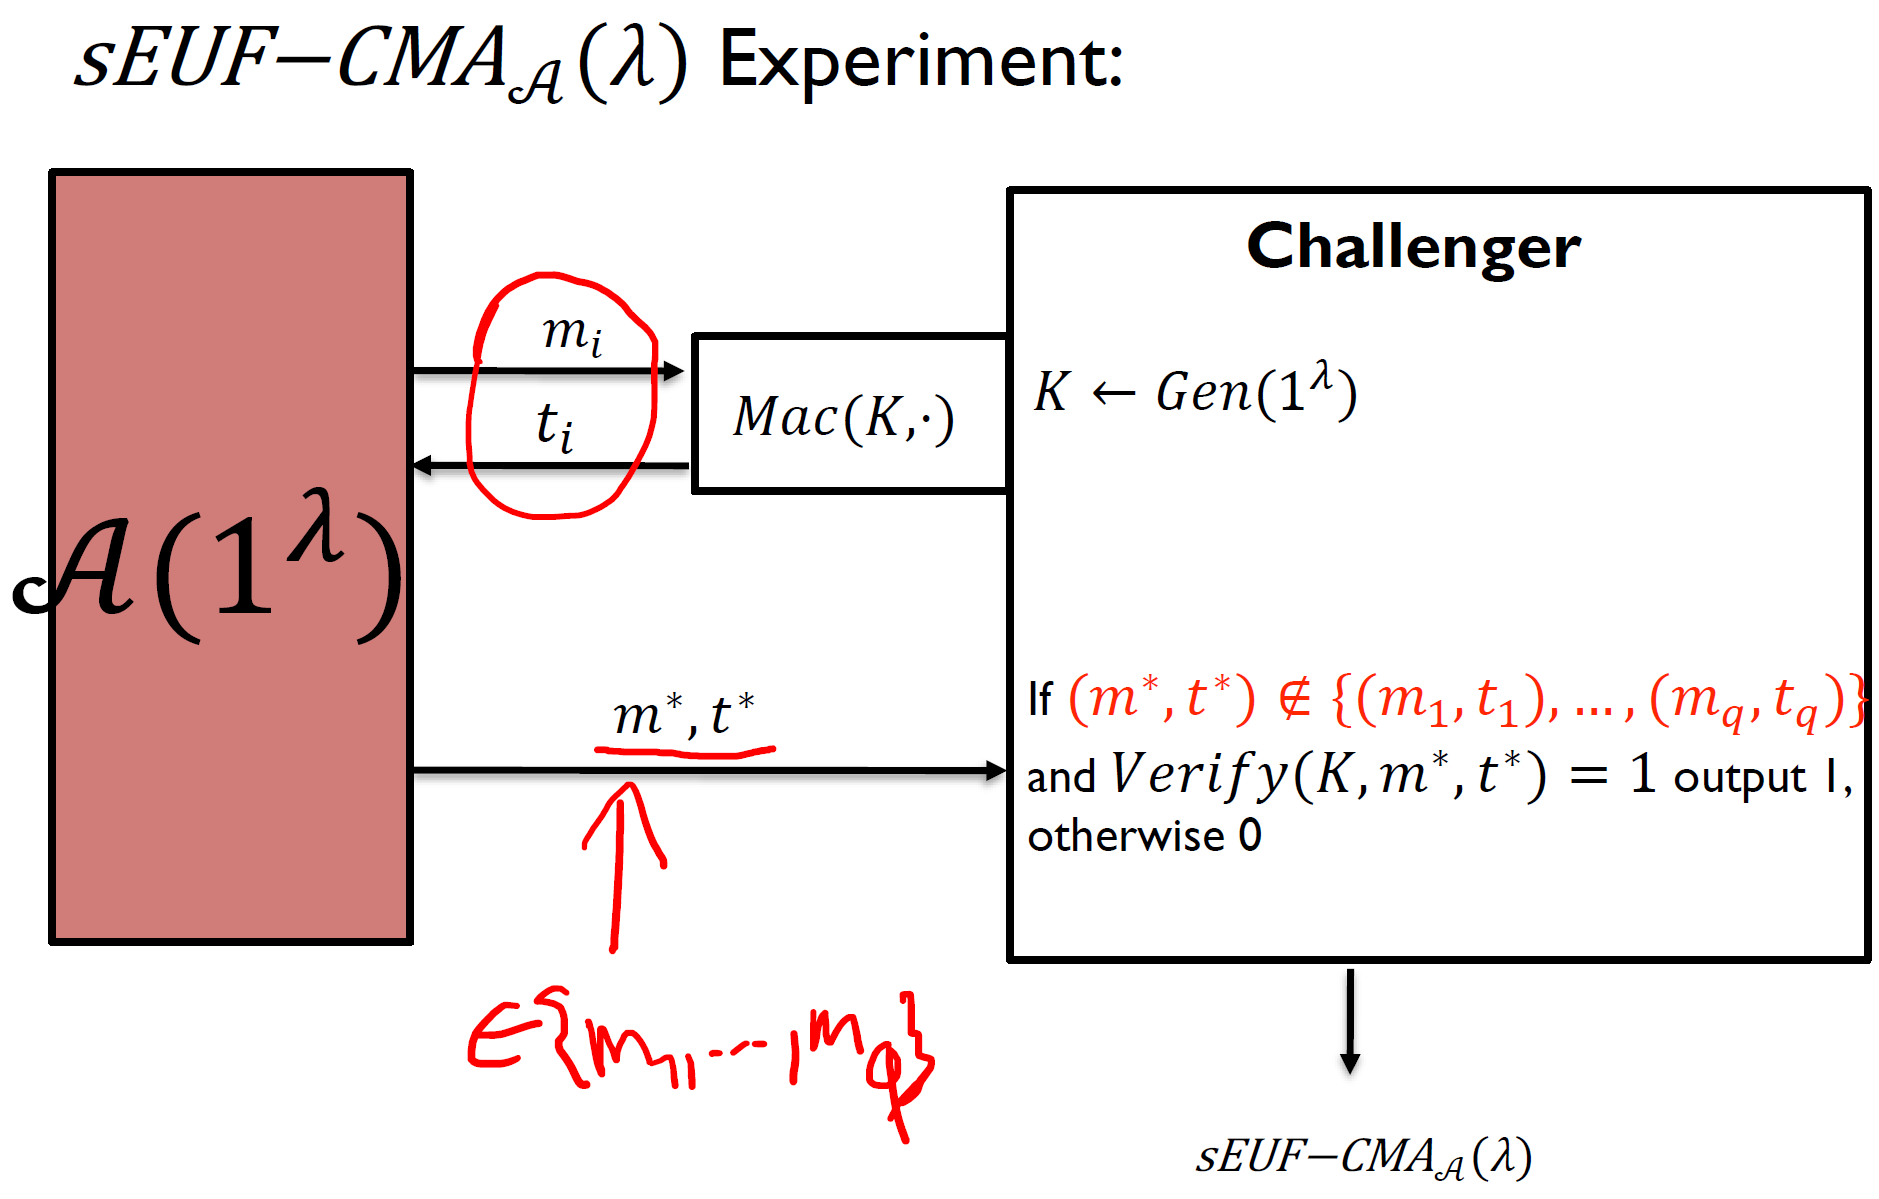
\includegraphics[width=120mm]{Graphics/Authentication/a4.png}
	\end{center}

\section{Using Message Authentication}
	\begin{center}
		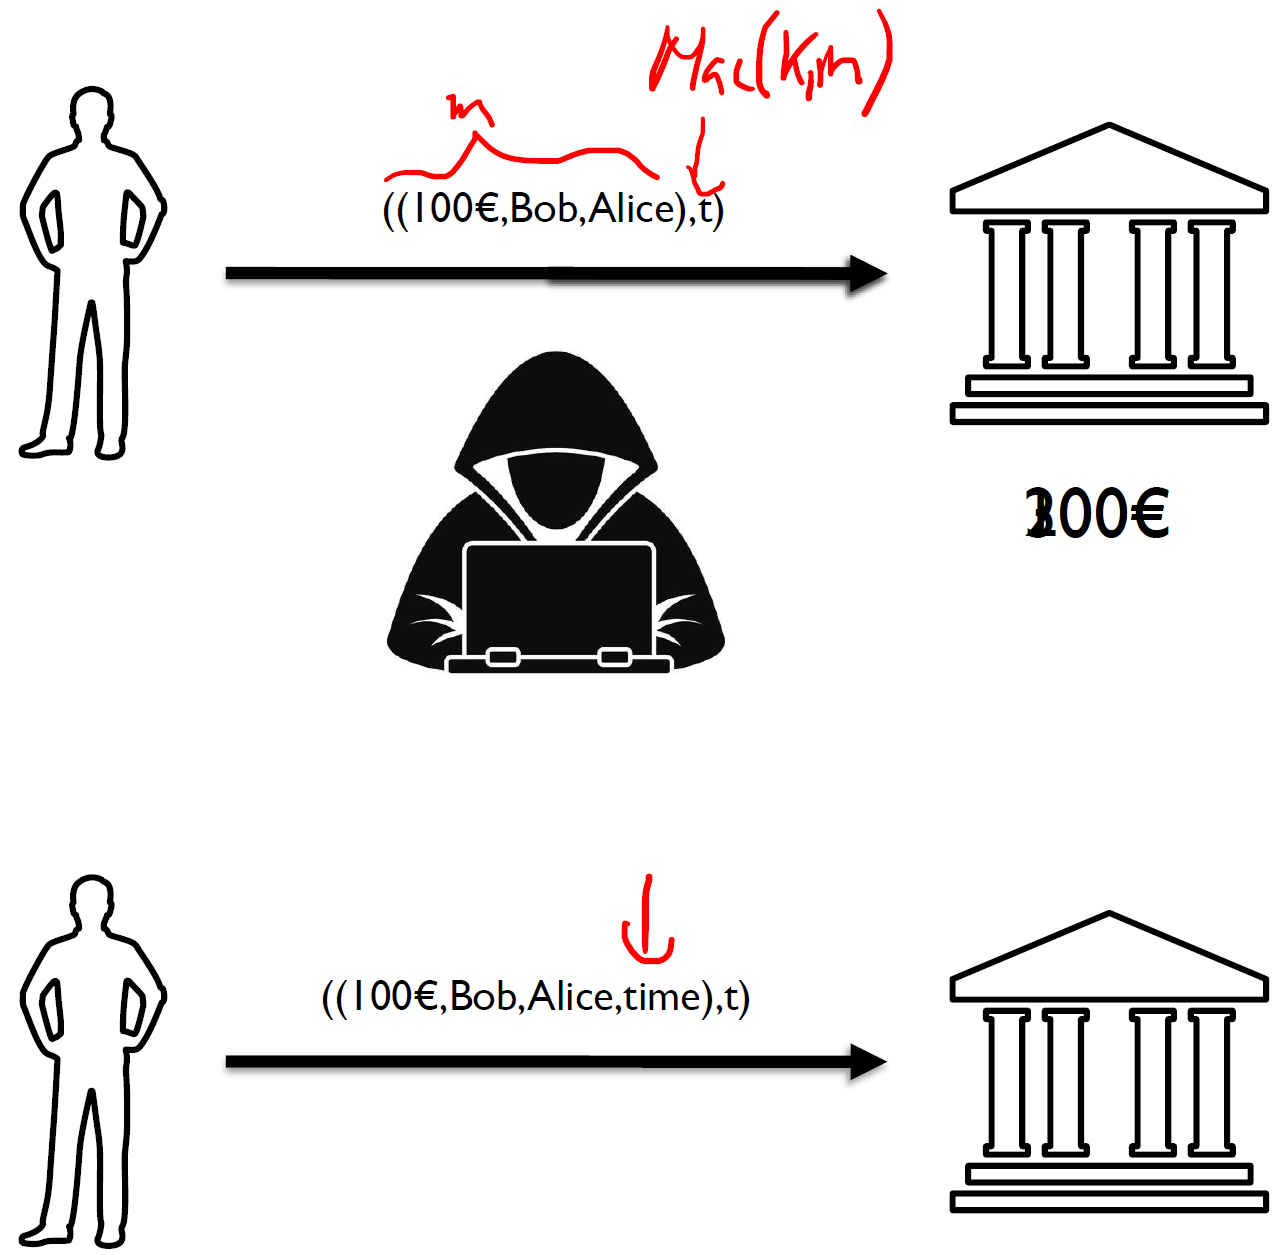
\includegraphics[width=120mm]{Graphics/Authentication/a5.png}
	\end{center}
	\begin{itemize}
		\item Message Authentication codes do not prevent replay attacks
		\item Need additional measures, e.g. timestamp
	\end{itemize}

\section{Summary 1}
	\begin{itemize}
		\item Message secrecy and message integrity are fundamentally different goals
		\item Encryption does not guarantee integrity
		\item Message Authentication Codes protect integrity of messages
		\item They don’t protect against replay attacks!
	\end{itemize}

\section{Constructing Message Authentication Codes}
	\begin{itemize}
		\item How should we construct MACs?
		\item Consider the constraints: Should not be possible to find an authentication tag for a new message
		\item What tools/primitives have we seen so far?
		\item We need a function which is unpredictable on new inputs
		\item ...the workhorse of symmetric key cryptography...
		\item ...pseudorandom functions!
	\end{itemize}
	
\section{Message Authentication Codes for fixed length messages}
	Assume for now we want to authenticate messages of fixed bit length $n$
	\textbf{Construction 6.1:}
	Let $PRF: \{0,1\}^{\lambda} \times \{0,1\}^{n} \rightarrow \{0,1\}^{\lambda}$ be a pseudorandom function
	\begin{itemize}
		\item $Gen(1^{\lambda})$: Choose key $K \leftarrow_{\$} \{0,1\}^{\lambda}$ for $PRF$
		\item $Mac(K,m)$: Compute $t \leftarrow PRF(K,m)$
		\item $Verify(K,m,t)$: If $t = PRF(K,m)$ output 1, otherwise 0
	\end{itemize}
	\textbf{Correctness:} Canonic

	\subsection{Security}
		\begin{theorem}\label{thm6.1}
			If $PRF$ is a pseudorandom function, then Construction 6.1 is a $sEUF-CMA$-secure $MAC$
		\end{theorem}
		\begin{proof}
			$MAC = (Gen,Mac,Verify)$ is not $EUF-CMA$-secure $\Rightarrow$ $PRF$ is not pseudorandom\\
			Let $\mathcal{A}$ be a $PPT$ adversary and $\epsilon$ a non-negligible function so that
			$$Pr[EUF-CMA_{\mathcal{A}}(\lambda) = 1] >\epsilon$$
			\begin{center}
				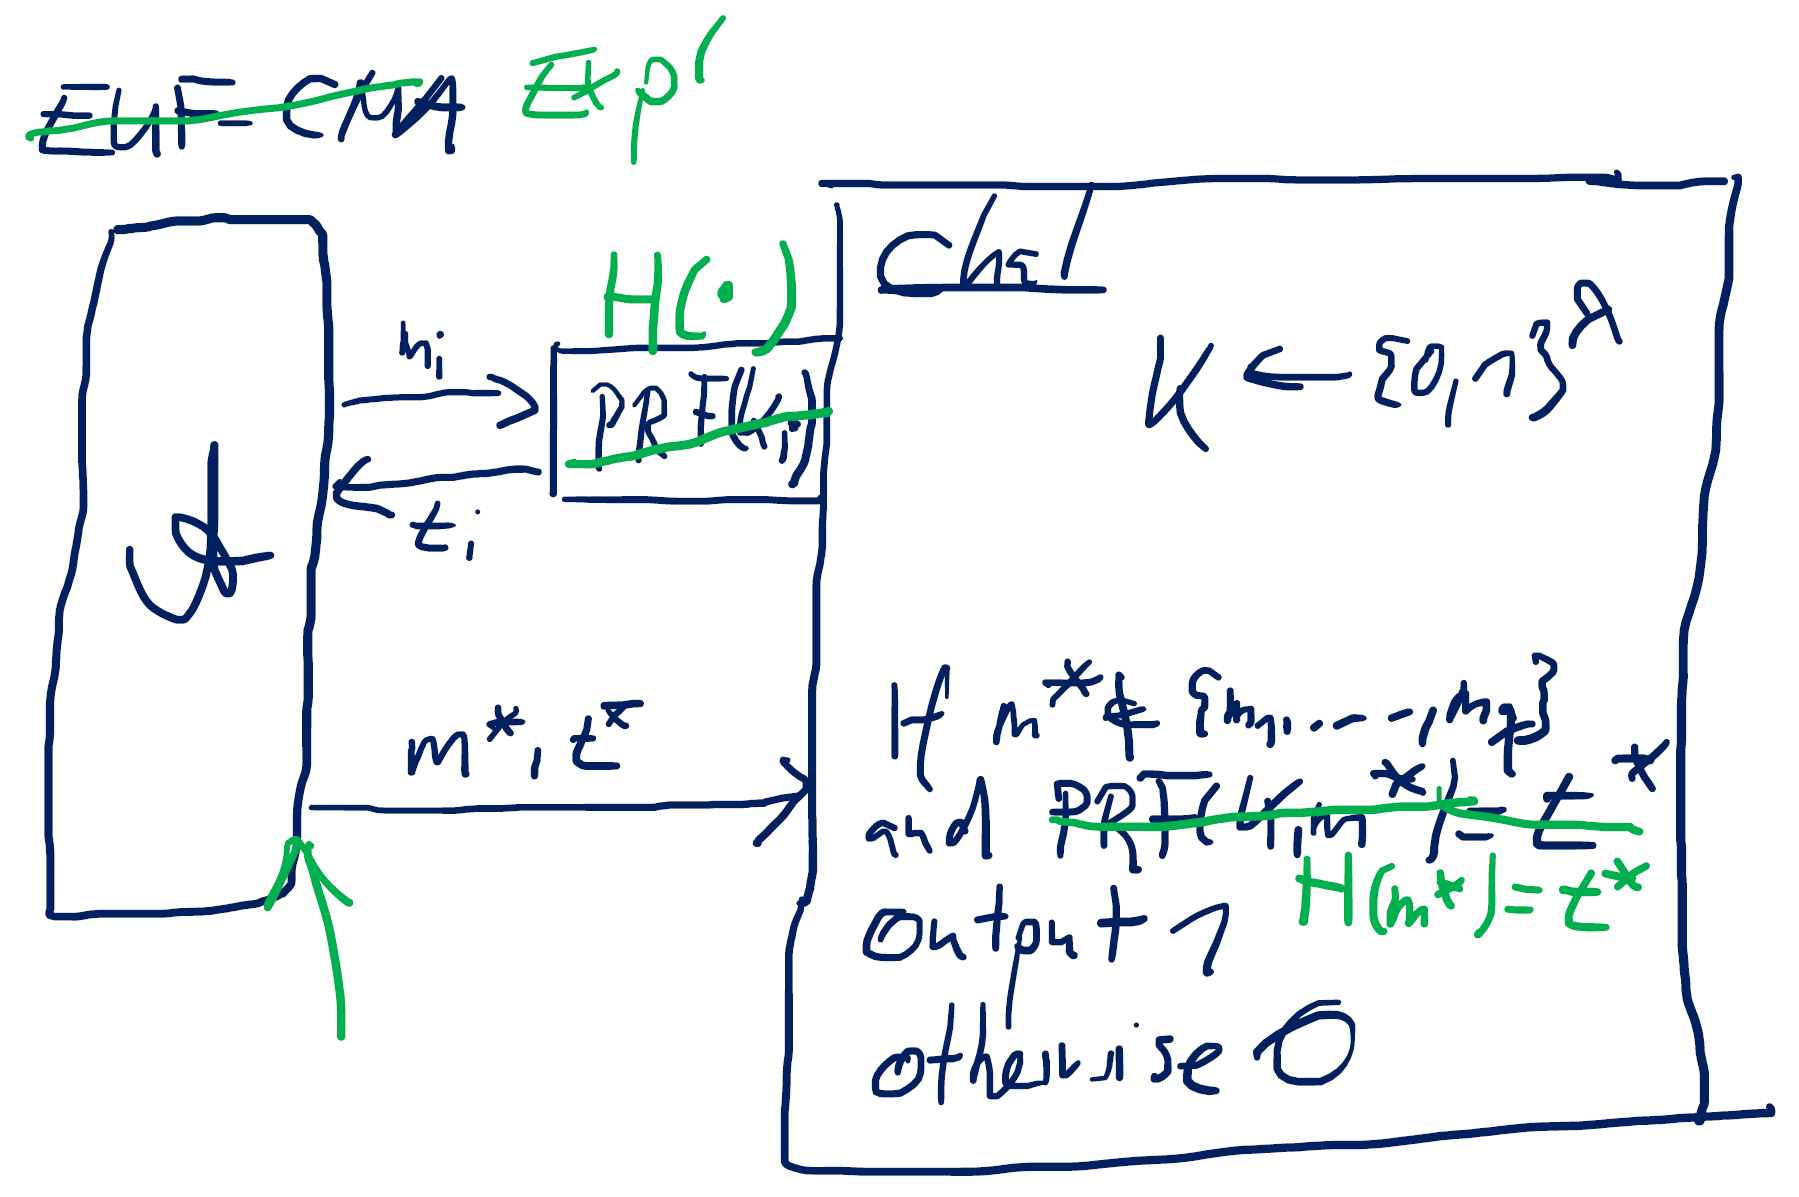
\includegraphics[width=140mm]{Graphics/Authentication/a6.png}
			\end{center}
			Assume $m^* \notin \{m_1,...,m_q\}$:
			\begin{itemize}
				\item $H$ is a truly random function
				\item $H(m^*)$ is uniformly random
				\item $Pr[H(m^*) = t^*] = 2^{-\lambda} (= \frac{1}{|\{0,1\}^{\lambda}|})$
				\item $Pr[Exp' = 1] 2^{-\lambda} \Rightarrow$ negligible!
			\end{itemize}
			\begin{center}
				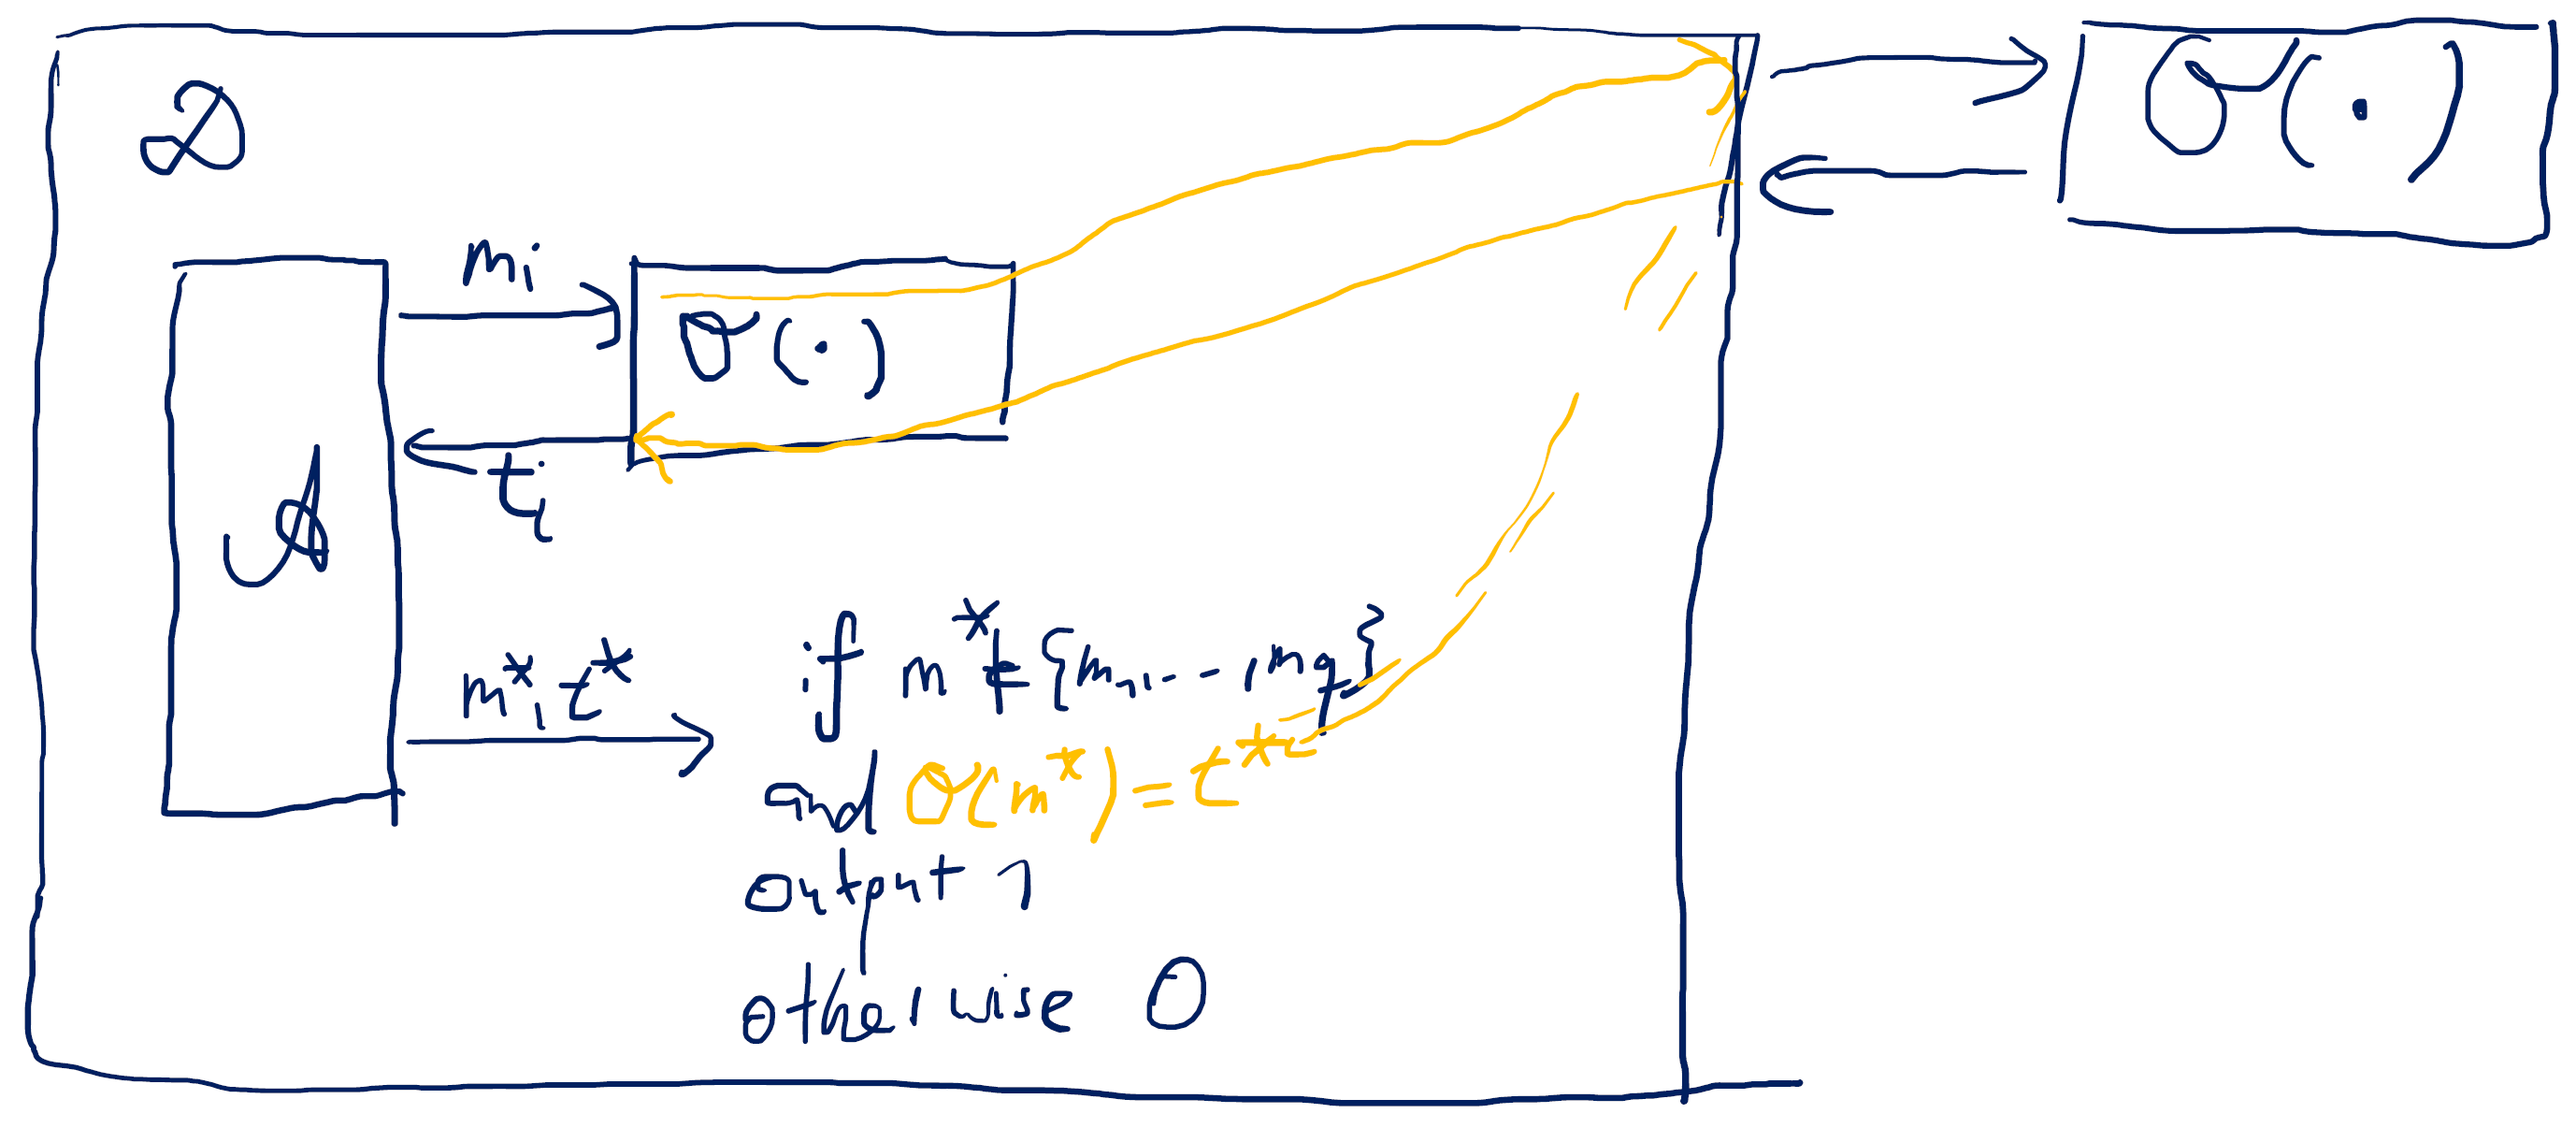
\includegraphics[width=140mm]{Graphics/Authentication/a7.png}
			\end{center}
			\underline{\textbf{Case 1:}} $\mathcal{O}(\cdot) = PRF(K,\cdot)$\\
			$\Rightarrow$ $\mathcal{D}$ perfectly simulates $EUF-CMA_{\mathcal{A}}(\lambda)$\\
			$\Rightarrow$ $Pr[\mathcal{D}^{PRF(K,\cdot)}(1^{\lambda}) = 1] = Pr[EUF-CMA_{\mathcal{A}}(\lambda) = 1] > \epsilon$\\
			\underline{\textbf{Case 2:}} $\mathcal{O}(\cdot) = H(\cdot)$\\
			$\Rightarrow$ $\mathcal{D}$ perfectly simulates $Exp'$\\
			$\Rightarrow$ $Pr[\mathcal{D}^{H(\cdot)}(1^{\lambda}) = 1] = Pr[Exp'_{\mathcal{A}}(\lambda) = 1] = 2^{-\lambda}$
			$$|Pr[\mathcal{D}^{PRF(K,\cdot)}(1^{\lambda}) = 1] - Pr[\mathcal{D}^{H(\cdot)}(1^{\lambda}) = 1]| > \epsilon - 2^{-\lambda}$$
			$\Rightarrow$ non-negligible!
		\end{proof}

\section{Message Authentication Codes for long Messages}
	\textbf{Construction 6.2:}
	Let $H: \{0,1\}^* \rightarrow \{0,1\}^{\lambda}$ be a hash function and $MAC = (Gen,Mac,Verify)$ be a message authentication code for messages of length $\lambda$.
	\begin{itemize}
		\item $Gen'(1^{\lambda})$: Generate $K' \leftarrow Gen(1^{\lambda})$ and $s \leftarrow_{\$} \{0,1\}^{\lambda}$. 
		Output $K = (s,K')$.
		\item $Mac'(K,m)$: Parse $K = (s,K')$.
		Compute and output $t \leftarrow MAC(K',H^s(m))$.
		\item $Verify'(K,m,t)$: If $t = MAC(K',H^s(m))$ output 1, otherwise 0.
	\end{itemize}
	\textbf{Correctness:} Canonic
	
	\subsection{Security}
		\begin{theorem}
			If $H$ is a collision resistant hash function and $MAC = (Gen,Mac,Verify)$ as $sEUF-CMA$-secure $MAC$, then $MAC' = (Gen',Mac',Verify')$ is a $sEUF-CMA$-secure $MAC$.
		\end{theorem}
		\begin{proof}
			\textbf{To show:}
			Assume $MAC'$ is not $EUF-CMA$ $\Rightarrow$ Either $H$ is not collision resistant or $MAC$ is not $EUF-CMA$-secure\\
			Let $\mathcal{A}$ be a PPT adversary and $\epsilon$ a non-negligible function so that
			$$Pr[EUF-CMA_{\mathcal{A}}^{MAC'}(\lambda) = 1] > \epsilon$$
			Set $Exp = EUF-CMA_{\mathcal{A}}^{MAC'}$
			\begin{center}
				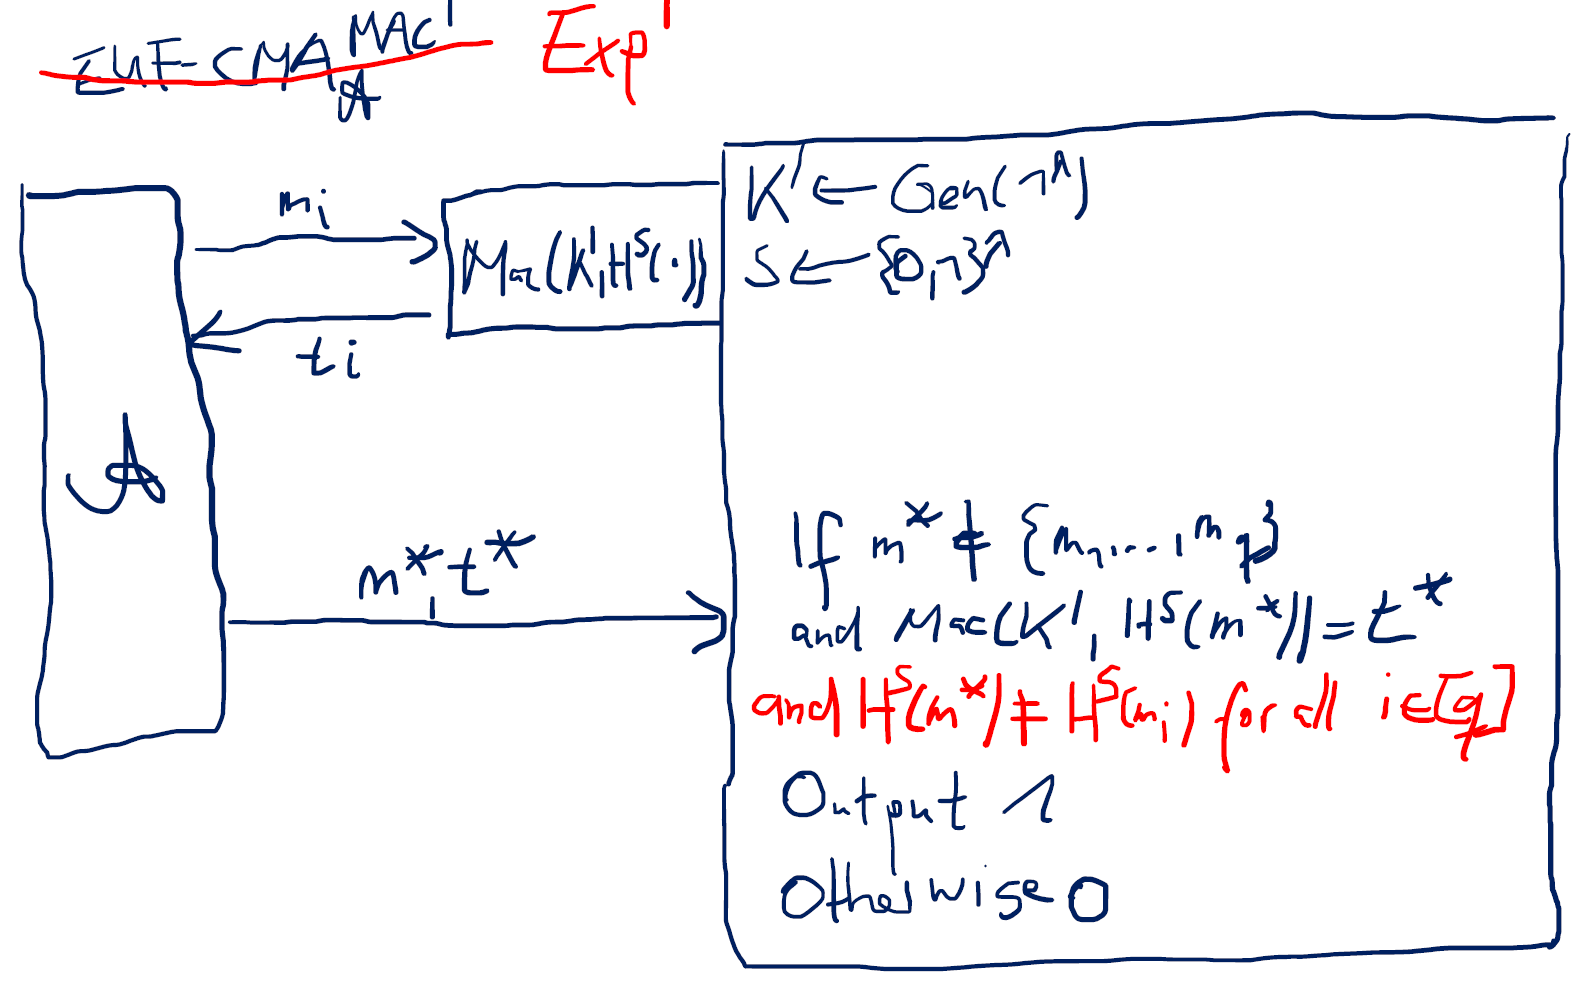
\includegraphics[width=140mm]{Graphics/Authentication/a8.png}
			\end{center}
			\underline{\textbf{Claim:}}
			$$|Pr[Exp = 1] - Pr[Exp' = 1]| < negl.$$
			Otherwise it is not collision resistant\\
			Proof via contraposition:\\
			Assume $|Pr[Exp = 1] - Pr[Exp' = 1]| > \epsilon'$ where $\epsilon'$ is non-negligible.\\
			\textbf{Observation:}
			If $H^s(m^*)$ does not collide with any of the $H^s(m_i)$ then the two experiments are identical.\\
			Let \underline{Col} be the event that $H^s(m^*) = H^s(m_i)$ for some $i \in [q]$ $m^* \neg m_i$\\
			With the LOTP it follows that
			\begin{enumerate}
				\item $Pr[Exp=1] = Pr[Exp=1 \mid Col] \cdot Pr[Col] + Pr[Exp=1 \mid \bar{Col}] \cdot Pr[\bar{Col}]$
				\item $Pr[Exp'=1] = Pr[Exp'=1 \mid Col] \cdot Pr[Col] + Pr[Exp'=1 \mid \bar{Col}] \cdot Pr[\bar{Col}]$
			\end{enumerate}
			With $Pr[Exp'=1 \mid Col]$ and $Pr[Exp=1 \mid Col] < 1$ we can consider
			$$\epsilon < Pr[Exp=1] - Pr[Exp'=1] = Pr[Exp=1 \mid Col] \cdot Pr[Col] < Pr[Col]$$
			\begin{center}
				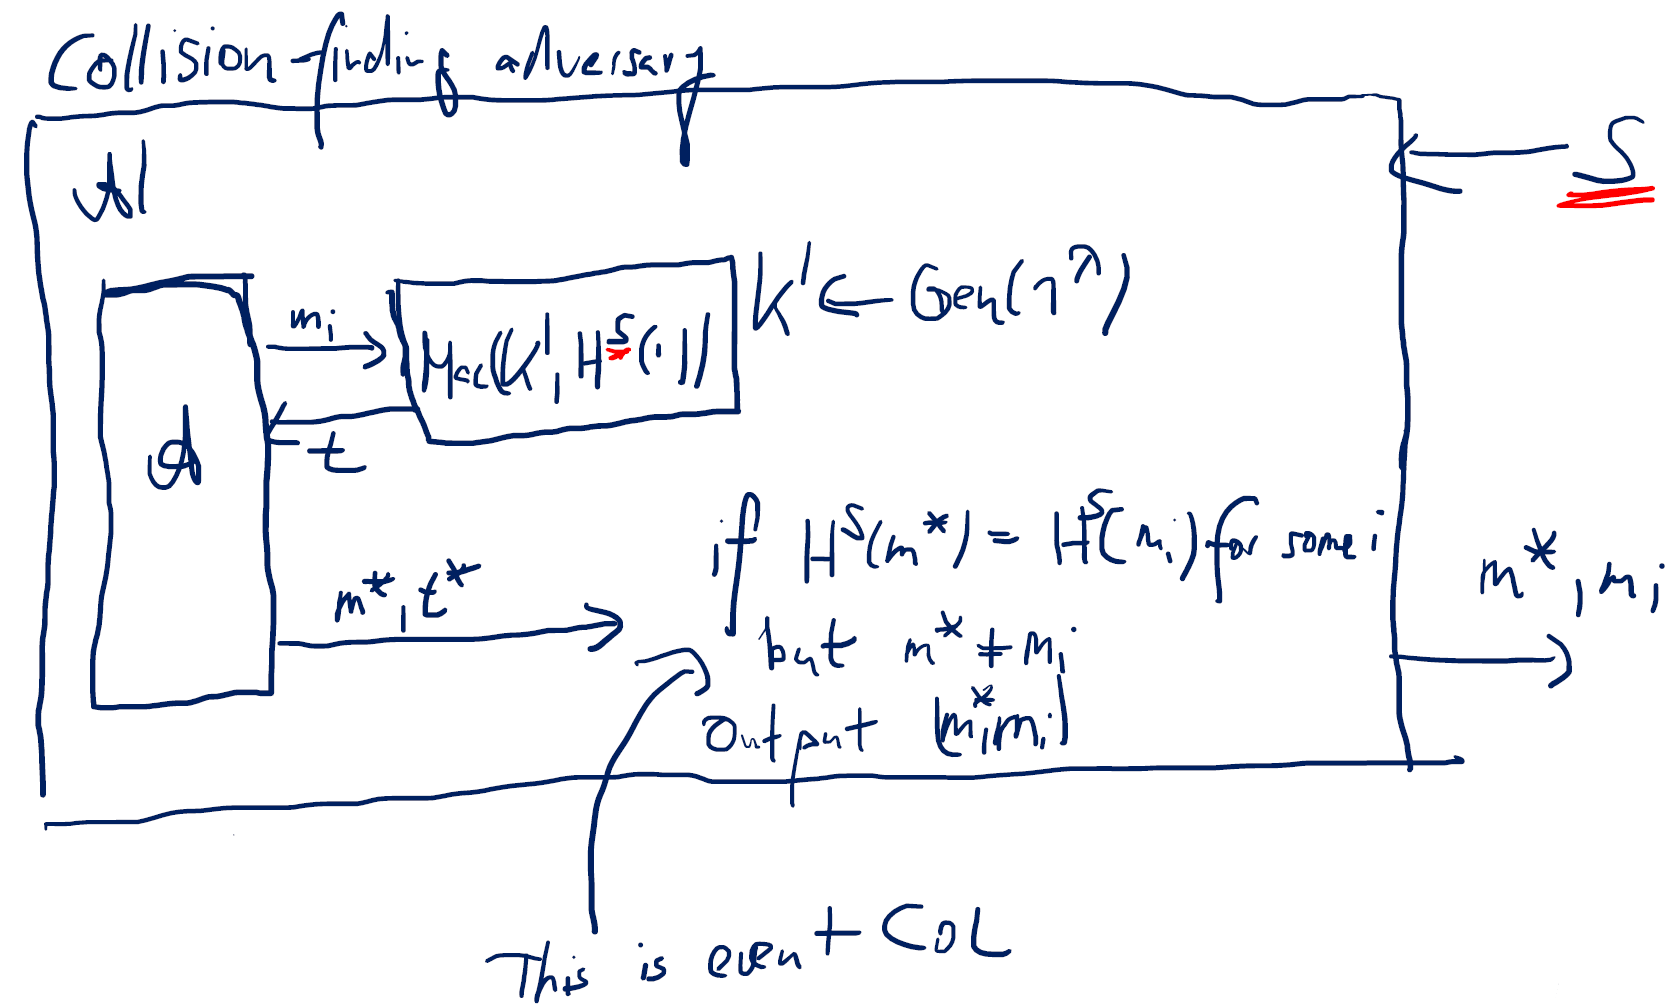
\includegraphics[width=140mm]{Graphics/Authentication/a9.png}
			\end{center}
			$$Pr[Hash-Col_{\mathcal{A}}(\lambda) = 1] = Pr[Col] > \epsilon'$$
			$\epsilon'$ is non-negligible. (Proves the Claim)\\
			Now assume $Pr[Exp=1]-Pr[Exp'=1] < negl.$ with $Pr[Exp=1] > \epsilon$\\
			$\Rightarrow$ $Pr[Exp'=1] > \epsilon - negl. = \epsilon'$ which is non-negligible.\\
			We will construct a PPT adversary $\mathcal{A}''$ against $MAC$
			\begin{center}
				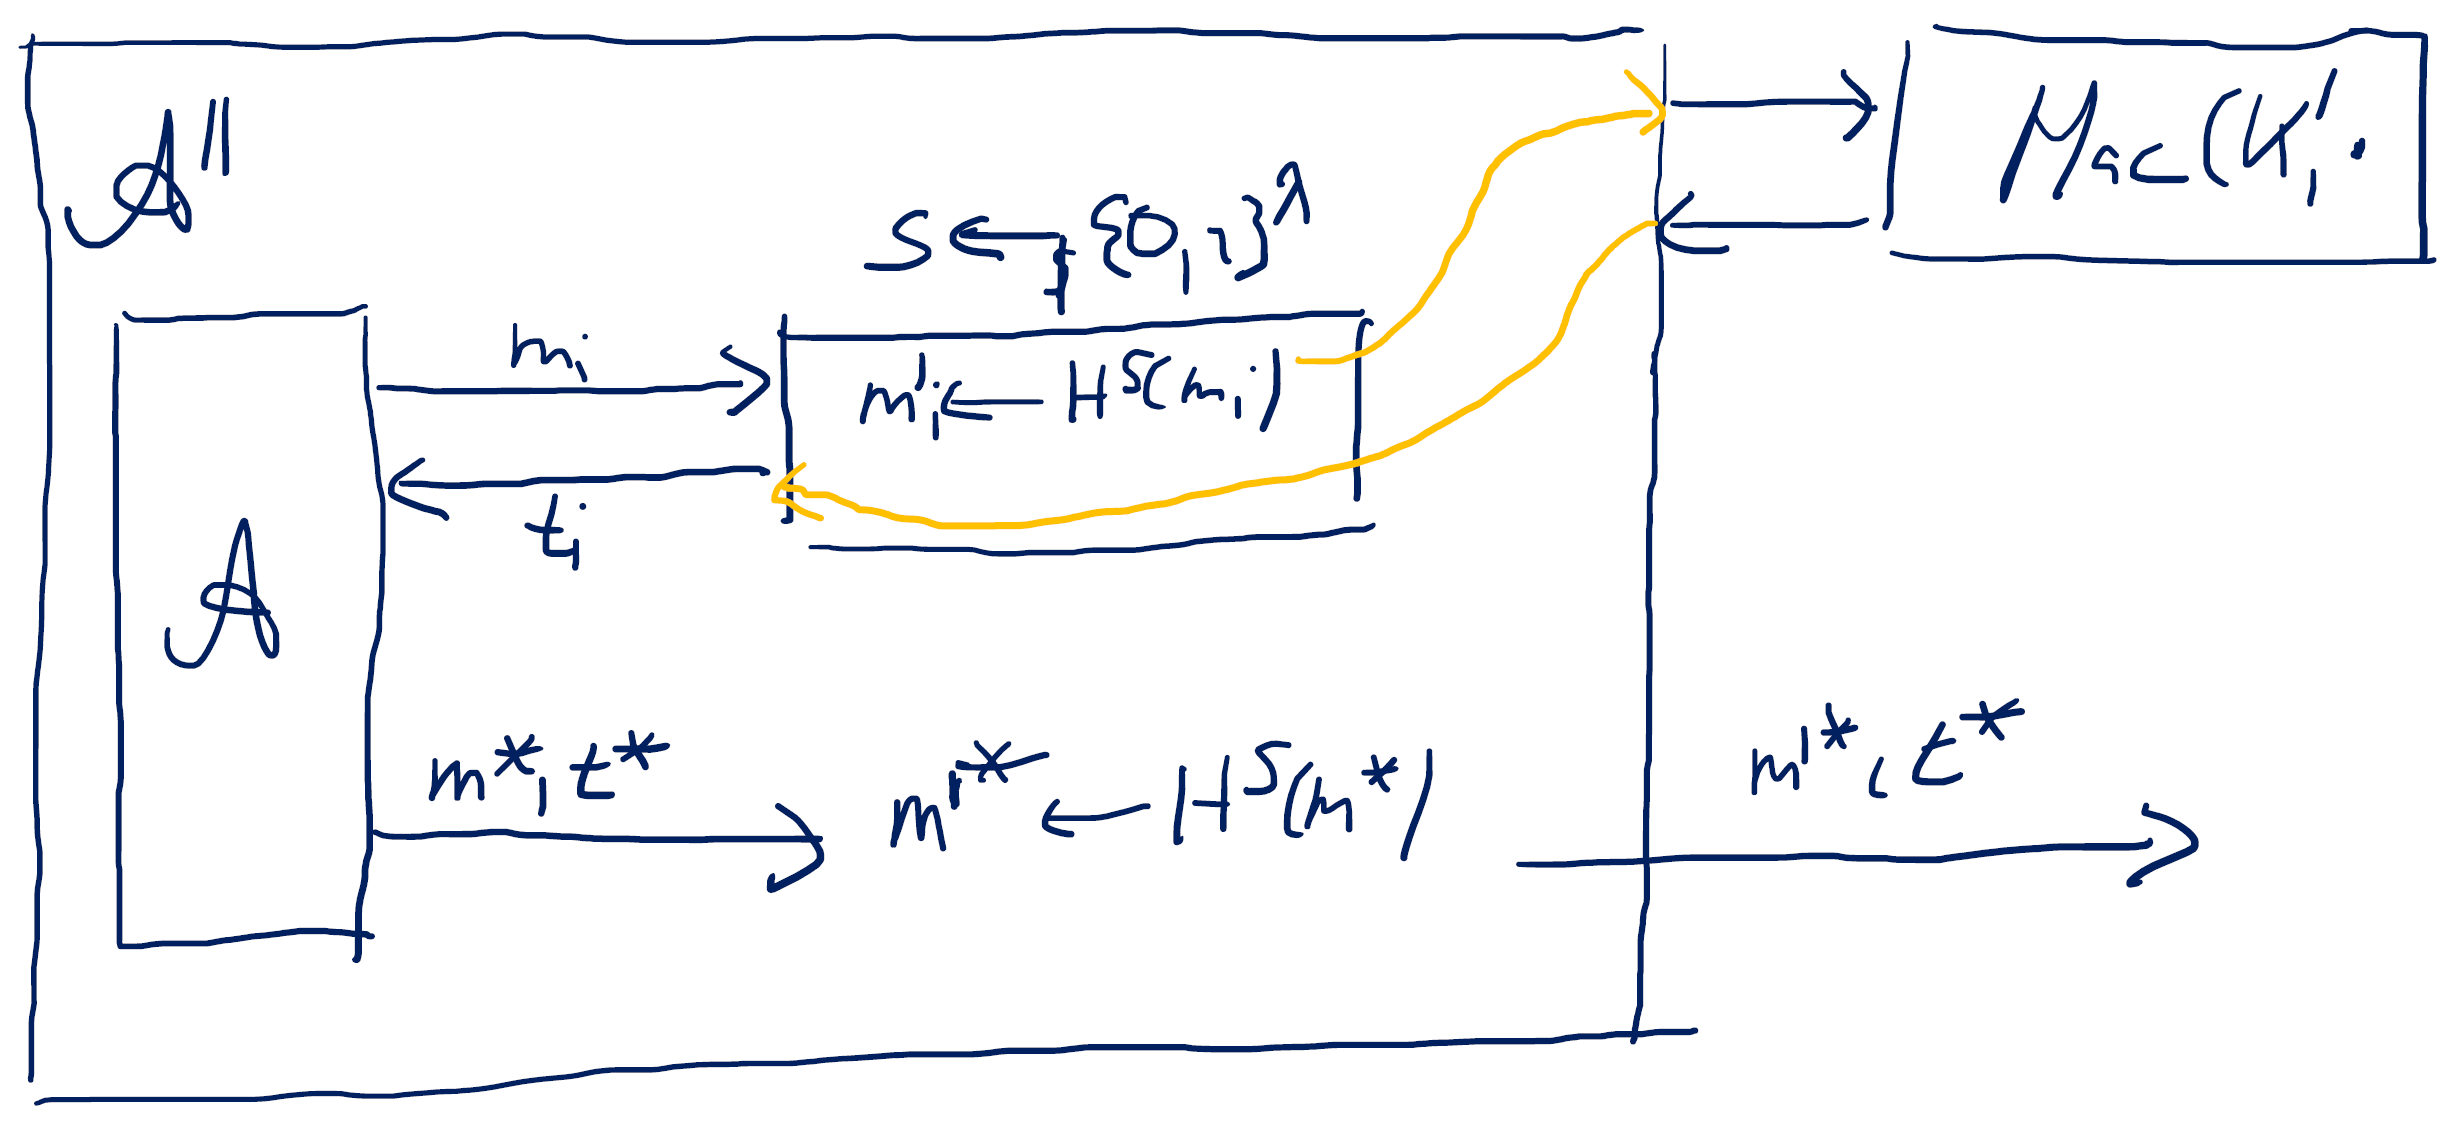
\includegraphics[width=140mm]{Graphics/Authentication/a10.png}
			\end{center}
			From the view of $\mathcal{A}$, $\mathcal{A}''$ simulates $Exp'$ perfectly
			$$Pr[EUF-CMA_{\mathcal{A}''}^{MAC}(\lambda) = 1] = Pr[Exp'_{\mathcal{A}} = 1] > \epsilon''$$
			which is non-negligible with $H^s(m^*) \neg H^s(m_i)$\\
			$\Rightarrow$ $m'^*$, $t^*$ is valid forge for $MAC$
		\end{proof}

\section{Message Authentication Codes from Random Oracles}
	\textbf{Construction 6.3:}
	Let $H: \{0,1\}^* \rightarrow \{0,1\}^{\lambda}$ be a hash function (modelled as a random oracle).
	\begin{itemize}
		\item $Gen(1^{\lambda})$: Generate $K \leftarrow_{\$} Gen(1^{\lambda})$. Output $K$.
		\item $Mac(K,m)$: Compute and output $t \leftarrow H(K||m)$.
		\item $Verify(K,m,t)$: If $t = H(K||m)$ output 1, otherwise 0.
	\end{itemize}
	\textbf{Correctness:} Canonic\\
	\textbf{Security:} $sEUF-CMA$ secure, proof essentially as in \cref{thm6.1}.\\
	
	\begin{itemize}
		\item However: Problematic when used with many practical hash functions!
		\item Merkle Damgård: $H(m_1||m_2||m_3) = h(h(m_1||m_2)||m_3)$
		\item $Mac(K,(m_1,m_2)) = H(K||m_1||m_2) = h(h(K||m_1)||m_2)$
	\end{itemize}

\section{Summary 2}
	\begin{itemize}
		\item MACs for fixed length messages can be constructed from PRFs
		\item Hash functions can be used to MAC messages of arbitrary length
		\item Random Oracles yield a simple MAC construction
		\item Be careful when a random oracle is replaced with a real hash function (Merkle Damgård)
	\end{itemize}


